\section{Fundamental objectives for foldings} \label{sec:objectives}

\subsection{Dihedral angles and Mountain/Valley assignments} \label{sec:dihedral}
\MiR{Straight and curved foldings are formed by rotating tangent vectors around the crease tangent. If the dihedral angle of the fold is $\alpha$, and initial tangents angle $t_1,t_2$ form an angle of $\beta$ with the tangent of the curve, then the angle formed is (write that down). Prescribing a dihedral angle can then be done by prescribing angles along the crease tangents. If the curve is straight than there is usually an extra degree of freedom for mountain-valley assignment. This also exists for one fold along a crease pattern. In that case we can use another constraint (write that down).}

\subsection{Controlling rulings} \label{sec:rulings}
\MiR{Explain about the importance of rulings in singularities and design in general. We don't necessarily want to fix them, but maybe fix some, or maybe force some condition of them such as being parallel (cylindrical) or avoid intersections in our domain.}
\subsubsection{Local rulings along a DOG} \label{sec:dog_rulings}
Let $f$ be a smooth parameterization of a developable surface. The second fundamental form of $f$, $II(v)$, can be written in coordinates $f_x,f_y$ as  $II(v)=v^tR^TDRv$, where:

\begin{equation} \label{second_smooth}
\begin{split}
R=\begin{pmatrix}cos(\theta) & -sin(\theta)\\
sin(\theta) &  cos(\theta)\\
\end{pmatrix},
D=\begin{pmatrix}0 & 0\\
0 &  2H\\
\end{pmatrix}
\end{split}
\end{equation}
Where $H$ is the mean curvature at the point, and $0 \leq \theta < \pi$ is the angle between the ruling of $f$ at the point and the tangent $f_x$. Let $k_x,k_y$ be the curvatures of the coordinate curves at the point. As seen in \cite{rabi2018shape}, if $f$ is an orthogonal geodesic net, $2H = k_x+k_y$, regardless of the angle between the principle curvatures and $k_x,k_y$. Similar to $H$, the angle to the ruling $\theta$ depends on the curvature of the coordinate curves:

\begin{theorem}
	\label{Lem:ruling_sym}
	Let $f$ be a smooth orthogonal geodesic net and let $k^x,k^y$ be the curvatures of the coordinate curves in directions $f_x,f_y$, then the angle $\theta$ satisfies:
	%
	\begin{equation}
	\tan(\theta) = \sqrt{\frac{k^x}{k^y}} \label{eq:rul_sym}
	\end{equation}
\end{theorem}
\proof{As the coordinate curves are geodesics, their curvature equals their normal curvature and so $k_x = II(f_x), k_y = II(f_y)$. Plugging $f_x \perp f_y$ into euler's formula we get $k_x = II(f_x) = 2Hsin^2(\theta) $ and $k_y = II(f_y) = 2Hcos^2(\theta)$.}\\
Determining the ruling directions in general require higher derivatives, the regularity of a smooth orthogonal net points at the ruling direction with lower derivatives, but up to symmetry as there are generally two possible values $\theta_1,\theta_2$ satisfying \eqref{eq:rul_sym} with $0 \leq \theta_1 \leq \frac{\pi}{2}$ and $ \theta_2 = \pi -\theta_1$.

\begin{topbot}
\begin{corollary}
\label{cor:cont_orth_geo_dev}
A smooth deformation on an orthogonal geodesic net fixes the ruling angles if and only if it keeps the ratio $\frac{k^x}{k^y}$ at any point.
\end{corollary}
\end{topbot}

\begin{topbot}
\begin{corollary}
\label{cor:cont_orth_geo_dev}
An orthogonal geodesic net $f$ is cylindrical, i.e. its rulings are parallel, if it satisfies $\frac{k^x}{k^y} = c$ for some constant $c$.
\end{corollary}
\end{topbot}


\subsubsection{Rulings along a crease} \label{sec:rulings_crease}
If the ruling angles of both surfaces along the crease are $\beta_1(t),\beta_2(t)$, measured by their angles with the tangents, then they satisfy the following \cite{more_on_paper,duncan_folded}:

\begin{equation}
\cot\beta_1(t) = \frac{\alpha'(t)-\tau(t)}{k(t)\sin(\alpha(t))},\cot\beta_2(t) = \frac{-\alpha'(t)-\tau(t)}{k(t)\sin(\alpha(t))}
\end{equation}
Which from here we can deduce (\cite{mathematical_omnibus,duncan_folded}):
\begin{equation} \label{cot_eq}
\begin{split}
\cot\beta_1(t) + \cot\beta_2(t) = \frac{-2\tau(t)}{k(t)\sin(\alpha(t))},\\
\cot\beta_1(t) - \cot\beta_2(t) = \frac{2\alpha'(t)}{k(t)\sin(\alpha(t))},
\end{split}	
\end{equation}
The authors of (\cite{mathematical_omnibus,duncan_folded}) identified two special cases, corresponding to when the above equations vanish. The first correspond to a planar curved fold, i.e. $\cot\beta_1(t) + \cot\beta_2(t) = \tau = 0$ which implies $\beta_1+\beta_2 = \pi$, meaning the rulings are continuation of each other on the flattened surface. In that case the two surfaces are just reflections of each other through the unique osculating plane of the curve (which doesn't change as $\tau = 0$). The second case corresponds to constant dihedral angle along the curve, i.e. $\cot\beta_1(t) - \cot\beta_2(t) = \alpha(t)' = 0$ which implies $\beta_1 = \beta_2$. These two cases coincide in the case $\beta_1 = \beta_2 = \frac{\pi}{2}$ (see \figref{fig:curved_different_rullings}).


\begin{figure} [h]
	\centering
	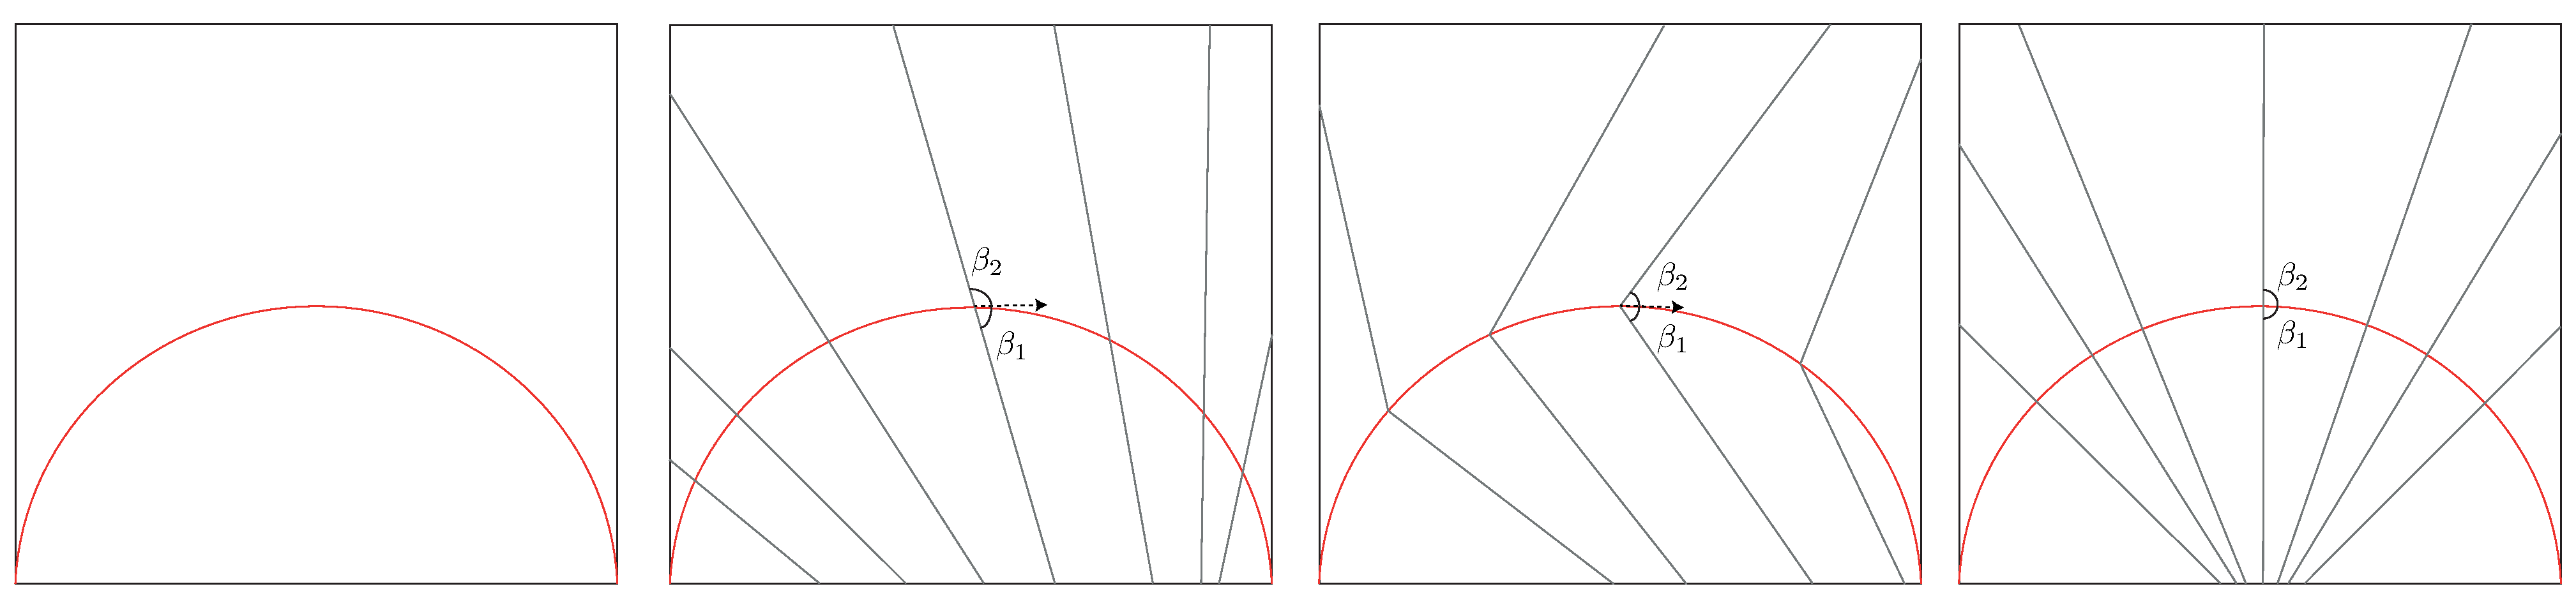
\includegraphics[width=\linewidth]{figures/curved_different_rullings}
	\caption{Different rulings patterns on a circular curved fold, displayed on the flattened configuration. From left to right: A circular curved fold pattern, a ruling pattern corresponding to $\beta_1(t)+\beta_2(t)=\pi$ (implying the curved fold is planar in 3D), a ruling pattern corresponding to $\beta_1(t)=\beta_2(t)$ (implying the dihedral angle between the tangent planes along the curve is constant) and a ruling pattern corresponding to both when $\beta_1(t)=\beta_2(t)=\frac{\pi}{2}$}
	\label{fig:curved_different_rullings}
\end{figure}

\subsection{Rulings objectives on DOG vertices}
